\subsection{Execution Contexts}
\label{sec:registers}

Application software targeting the 64-bit Intel architecture uses a variety of
CPU registers to interact with the processor's features, shown in
Figure~\ref{fig:cpu_registers} and Table~\ref{fig:xsave_state}. The values in
these registers make up an application thread's state, or \textit{execution
context}.

OS kernels multiplex each logical processor (\S~\ref{sec:cpu_core}) between
multiple software threads by \textit{context switching}, namely saving the
values of the registers that make up a thread's execution context, and
replacing them with another thread's previously saved context. Context
switching also plays a part in executing code inside secure containers, so its
design has security implications.

% 64-Bit Mode Execution Environment: SDM vol1 S 3.2.1
% Basic Program Execution Registers: SDM vol1 S 3.4

\begin{figure}[hbt]
  \centering
  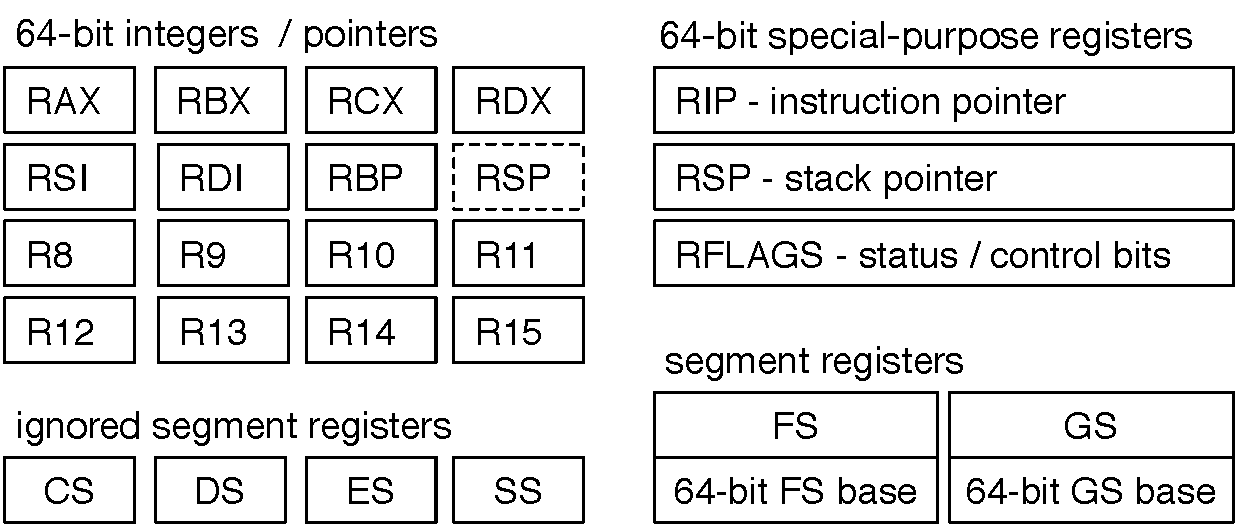
\includegraphics[width=85mm]{figures/cpu_registers.pdf}
  \caption{
    CPU registers in the 64-bit Intel architecture. RSP can be used as a
    general-purpose register (GPR), e.g., in pointer arithmetic, but it always
    points to the top of the program's stack. Segment registers are covered in
    \S~\ref{sec:segments}.
  }
  \label{fig:cpu_registers}
\end{figure}

Integers and memory addresses are stored in 16 \textit{general-purpose
registers} (GPRs). The first 8 GPRs have historical names: RAX, RBX, RCX,
RDX, RSI, RDI, RSP, and RBP, because they are extended versions of the 32-bit
Intel architecture's GPRs. The other 8 GPRs are simply known as R9-R16. RSP is
designated for pointing to the top of the procedure call stack, which is simply
referred to as \textit{the stack}. RSP and the stack that it refers to are
automatically read and modified by the CPU instructions that implement
procedure calls, such as \texttt{CALL} and \texttt{RET} (return), and by
specialized stack handling instructions such as \texttt{PUSH} and \texttt{POP}.

All applications also use the RIP register, which contains the address of the
currently executing instruction, and the RFLAGS register, whose bits (e.g.,
the carry flag - CF) are individually used to store comparison results and
control various instructions.

% XSAVE-Supported Features and State-Component Bitmaps: SDM vol1 S 13.1
% Enabling the XSAVE Feature Set and XSAVE-Enabled Features: SDM vol1 S13.3
% XSAVE-managed State: SDM vol1 S 13.5

Software might use other registers to interact with specific processor
features, some of which are shown in Table~\ref{fig:xsave_state}.

\begin{table}[hbt]
  \centering
  \begin{tabularx}{\columnwidth}{| l | X | l |}
  \hline
  \textbf{Feature} & \textbf{Registers} & \textbf{XCR0 bit}\\
  \hline
  FPU & FP0 - FP7, FSW, FTW & 0 \\
  \hline
  SSE & MM0 - MM7, XMM0 - XMM15, XMCSR & 1 \\
  \hline
  AVX & YMM0 - YMM15 & 2 \\
  \hline
  AVX-512 & K0 - K7 & 5 \\
  \hline
  AVX-512 & ZMM0\_H  - ZMM15\_H & 6 \\
  \hline
  AVX-512 & ZMM16 - ZMM31 & 7 \\
  \hline
  PK & PKRU & 9 \\
  \hline
  \end{tabularx}
  \caption{Sample feature-specific Intel architecture registers.}
  \label{fig:xsave_state}
\end{table}

The Intel architecture provides a future-proof method for an OS kernel to save
the values of feature-specific registers used by an application. The
\texttt{XSAVE} instruction takes in a bitmap of features, and writes the
registers used by the features whose bits are set to 1 in a memory area that
can be used by the \texttt{XRSTOR} instruction to load the saved values back
into feature-specific registers.

Application software declares the features that it plans to use to the kernel,
so the kernel knows what XSAVE bitmap to use when context-switching. When
receiving the system call, the kernel sets the XCR0 register to the feature
bitmap declared by the application. The CPU generates a fault if application
software attempts to use features that are not enabled by XCR0, so applications
cannot modify feature-specific registers that the kernel wouldn't take into
account when context-switching. The kernel can use the \texttt{CPUID}
instruction to learn the size of the XSAVE memory area for a given feature
bitmap, and compute how much memory it needs to allocate for the context of
each of the application's threads.
